%
% File tupa_multilingual.tex

\documentclass[11pt,a4paper]{article}
\usepackage[hyperref]{emnlp2018}
\usepackage{times}
\usepackage{latexsym}
\usepackage{amsmath}
\usepackage{tikz}
\usepackage{tikz-dependency}
\usepackage[warn]{textcomp}
\usepackage[font=small]{caption}
\usepackage{subcaption}
\usepackage{multirow}
\usepackage{url}
\usepackage{etoolbox}
\usepackage{xr}

\newcommand{\com}[1]{}
\newcommand{\oa}[1]{\footnote{\color{red}OA: #1}}
\newcommand{\daniel}[1]{\footnote{\color{blue}Daniel: #1}}

\hyphenation{SemEval}

\DeclareMathOperator*{\argmin}{argmin}
\DeclareMathOperator*{\argmax}{argmax}

\makeatletter
\patchcmd\@combinedblfloats{\box\@outputbox}{\unvbox\@outputbox}{}{%
   \errmessage{\noexpand\@combinedblfloats could not be patched}%
}%
 \makeatother


\usetikzlibrary{shapes,shapes.misc}

%\aclfinalcopy % Uncomment this line for the final submission
\def\aclpaperid{600}

%\setlength\titlebox{5cm}
% You can expand the titlebox if you need extra space
% to show all the authors. Please do not make the titlebox
% smaller than 5cm (the original size); we will check this
% in the camera-ready version and ask you to change it back.

\title{Multilingual UCCA Parsing}

\author{Daniel Hershcovich$^{1,2}$ \\
  \\\And
  Omri Abend$^2$ \\
  $^1$The Edmond and Lily Safra Center for Brain Sciences \\
  $^2$School of Computer Science and Engineering \\
  Hebrew University of Jerusalem \\
  \texttt{\{danielh,oabend,arir\}@cs.huji.ac.il}
  \\\And
  Ari Rappoport$^2$
}

\date{}

\begin{document}

\maketitle

\begin{abstract}
\end{abstract}

\section{Introduction}\label{sec:introduction}


%%%%%%%%%%%%%%%%%%%%%%%%%%%%%%%%%%%%%%%%%%%%%%%%%%%%%%%%%%%%%%%%%%%%%%%%%%%%%%%%%
\section{Related Work}\label{sec:related_work}

\begin{figure}[!ht]
\fbox{\begin{subfigure}{0.47\textwidth}
  \centering
  \scalebox{.95}{
  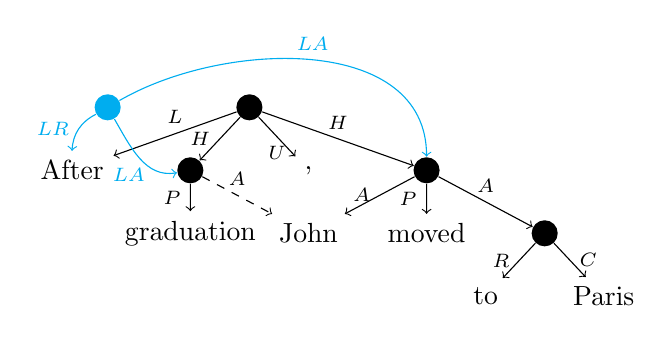
\begin{tikzpicture}[level distance=8mm, ->]
    \node (ROOT) [fill=black, circle] {}
      child {node (After) {After} edge from parent node[above] {\scriptsize $L$}}
      child {node (graduation) [fill=black, circle] {}
      {
        child {node {graduation} edge from parent node[left] {\scriptsize $P$}}
      } edge from parent node[left] {\scriptsize $H$} }
      child {node {,} edge from parent node[below] {\scriptsize $U$}}
      child {node (moved) [fill=black, circle] {}
      {
        child {node (John) {John} edge from parent node[left] {\scriptsize $A$}}
        child {node {moved} edge from parent node[left] {\scriptsize $P$}}
        child {node [fill=black, circle] {}
        {
          child {node {to} edge from parent node[left] {\scriptsize $R$}}
          child {node {Paris} edge from parent node[right] {\scriptsize $C$}}
        } edge from parent node[above] {\scriptsize $A$} }
      } edge from parent node[above] {\scriptsize $H$} }
      ;
    \draw[dashed,->] (graduation) to node [above] {\scriptsize $A$} (John);
    \node (LKG) at (-1.8,0) [fill=cyan, circle] {};
    \draw[bend right,color=cyan] (LKG) to node [auto, left] {\scriptsize $LR$} (After);
    \draw[color=cyan] (LKG) to[out=-60, in=190] node [below] {\scriptsize $LA\quad$} (graduation);
    \draw[color=cyan] (LKG) to[out=30, in=90] node [above] {\scriptsize $LA$} (moved);
  \end{tikzpicture}
  }\caption{UCCA \label{fig:original_example_ucca}}
\end{subfigure}}

\caption{\label{fig:original_examples}}

\end{figure}


%%%%%%%%%%%%%%%%%%%%%%%%%%%%%%%%%%%%%%%%%%%%%%%%%%%%%%%%%%%%%%%%%%%%%%%%%%%%%%%%%

\paragraph{Universal Conceptual Cognitive Annotation.}\label{sec:ucca}
UCCA \cite{abend2013universal} is a semantic representation whose main design principles
are ease of annotation, cross-linguistic applicability, and a modular architecture.
%of semantic distinctions.
UCCA represents the semantics of linguistic utterances
as directed acyclic graphs (DAGs), where terminal (childless) nodes
correspond to the text tokens, and non-terminal nodes to semantic units that participate
in some super-ordinate relation.
Edges are labeled, indicating the role of a child in the relation the parent represents.
Nodes and edges belong to one of several \textit{layers}, each corresponding
to a ``module'' of semantic distinctions.
UCCA's \textit{foundational layer} (the only layer for which annotated data exists)
mostly covers predicate-argument structure, semantic heads and inter-Scene relations.
%The \textit{linkage} layer covers relations between events, including temporal and discourse relations
%(exemplified by the gray node and its outgoing edges in Figure~\ref{fig:original_example_ucca}).

UCCA distinguishes \textit{primary} edges, corresponding 
to explicit relations, from \textit{remote} edges (appear dashed in
Figure~\ref{fig:original_example_ucca}) that allow for a unit to participate
in several super-ordinate relations.
Primary edges form a tree in each layer, whereas remote edges enable reentrancy, forming a DAG.
%As UCCA annotated data is currently fairly scarce (see \S\ref{sec:experiments}), 
%we hypothesize it will benefit from MTL, and consider it as our
%main task.


\subsection{TUPA's Transition Set}\label{sec:transition_set}

Given a sequence of tokens $w_1, \ldots, w_n$,
we predict a rooted graph $G$ whose terminals are the tokens.
Parsing starts with the root node on the stack,
and the input tokens in the buffer.

The TUPA transition set includes
the standard \textsc{Shift} and \textsc{Reduce} operations,
\textsc{Node$_X$} for creating a new non-terminal node and an $X$-labeled edge,
\textsc{Left-Edge$_X$} and \textsc{Right-Edge$_X$} to create a new primary $X$-labeled edge,
\textsc{Left-Remote$_X$} and \textsc{Right-Remote$_X$} to create a new remote $X$-labeled edge,
\textsc{Swap} to handle discontinuous nodes,
and \textsc{Finish} to mark the state as terminal.

Although UCCA contains nodes without any text tokens as descendants
(called \textit{implicit units}),
these nodes are infrequent and only cover 0.5\% of non-terminal nodes.
For this reason we follow previous work \cite{hershcovich2017a} and discard implicit units from
the training and evaluation,
and so do not include transitions for creating them.

\begin{figure}[t]
   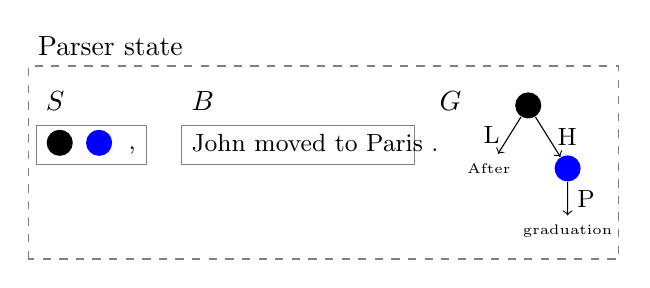
\begin{tikzpicture}[level distance=8mm, sibling distance=1cm]
   \node[anchor=west] at (0,1.5) {Parser state};
   \draw[color=gray,dashed] (0,-1.2) rectangle (7.5,1.25);
   \draw[color=gray] (.1,0) rectangle (1.5,.5);
   \node[anchor=west] at (.1,.8) {$S$};
   \node[fill=black, circle] at (.4,.275) {};
   \node[fill=blue, circle] at (.9,.275) {};
   \node[anchor=west] at (1.15,.175) {\small ,};
   \draw[color=gray] (1.95,0) rectangle (4.9,.5);
   \node[anchor=west] at (1.95,.8) {$B$};
   \node[anchor=west] at (1.95,.275) {\small John moved to Paris .};
   \node[anchor=west] at (5.1,.8) {$G$};
   \node[fill=black, circle] at (6.35,.75) {}
     child {node  {\tiny After} edge from parent [->] node[left] {\small L}}
     child {node [fill=blue, circle] {}
     {
       child {node {\tiny graduation} edge from parent [->] node[right] {\small P}}
     } edge from parent [->] node[right] {\small H} };
   \end{tikzpicture}
   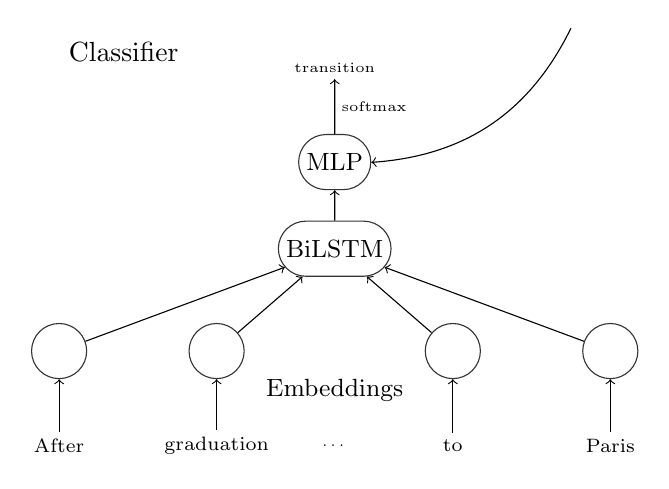
\begin{tikzpicture}[->]
   \node[anchor=west] at (0,6) {Classifier};
   \tiny
   \tikzstyle{main}=[rounded rectangle, minimum size=7mm, draw=black!80, node distance=12mm]
   \node[main] (specific) at (3.5,3.5) {\small BiLSTM};
   \node (embeddings) at (3.5,1.7) {\small Embeddings};
   \foreach \i/\word in {0/{After},2/{graduation},5/{to},7/{Paris}} {
       \node (x\i) at (\i,1) {\scriptsize \word};
       \node[main] (e\i) at (\i,2.2) {};
       \path (x\i) edge (e\i);
       \path (e\i) edge (specific);
   }
    \node (x4) at (3.5,1) {\ldots};
    \node[main] (mlp) at (3.5,4.6) {\small MLP};
    \path (specific) edge (mlp);
    \coordinate (state) at (6.5,6.3);
    \path (state) edge [bend left] (mlp);
    \node (transition) at (3.5,5.8) {transition};
    \path (mlp) edge node[right] {softmax} (transition);
   \end{tikzpicture}
\caption{Illustration of the TUPA model, adapted (with permission) from \citet{hershcovich2017a}.
Top: parser state.
Bottom: BiLTSM architecture.}\label{fig:single_model}
\end{figure}


%%%%%%%%%%%%%%%%%%%%%%%%%%%%%%%%%%%%%%%%%%%%%%%%%%%%%%%%%%%%%%%%%%%%%%%%%%%%%%%%%
\subsection{Transition Classifier}\label{sec:classifier}

To predict the next transition at each step,
we use a BiLSTM with embeddings as inputs,
followed by an MLP and a softmax layer for classification \cite{kiperwasser2016simple}.
The model is illustrated in Figure~\ref{fig:single_model}.
Inference is performed greedily,
and training is done with an oracle that yields the set of all optimal 
transitions at a given state (those that lead to a state from which the gold graph is still reachable).
Out of this set, the actual transition performed in training is the one
with the highest score given by the classifier,
which is trained to maximize the sum of log-likelihoods of all 
optimal transitions at each step.


\paragraph{Features.}
We use the original TUPA features,
representing the words, POS tags, syntactic dependency relations, and previously predicted edge labels
for nodes in specific locations in the parser state.
In addition, for each token
we use embeddings representing the one-character prefix, three-character suffix,
shape (capturing orthographic features, e.g., ``Xxxx''),
and named entity type,\footnote{See Supplementary Material for a full listing of features.}
all provided by spaCy \cite{spacy2}.\footnote{\url{http://spacy.io}}
To the learned word vectors, we concatenate the 250K most frequent word vectors from fastText
\cite{bojanowski2016enriching},\footnote{\url{http://fasttext.cc}}
pre-trained over Wikipedia and updated during training.



%%%%%%%%%%%%%%%%%%%%%%%%%%%%%%%%%%%%%%%%%%%%%%%%%%%%%%%%%%%%%%%%%%%%%%%%%%%%%%%%%%%%%%%%%%%%
\section{Multilingual Transition-based Parsing}\label{sec:multitask}



\section{Experiments}\label{sec:experiments}

\begin{table*}[t]
\centering
\small
\setlength\tabcolsep{2pt}
\begin{tabular}{l|ccc|ccc||ccc|ccc||ccc|ccc}
& \multicolumn{6}{c||}{\footnotesize \bf English}
& \multicolumn{6}{c||}{\footnotesize \bf French}
& \multicolumn{6}{c}{\footnotesize \bf German} \\
\hline
& \multicolumn{3}{c|}{\footnotesize \bf {\#} tokens}
& \multicolumn{3}{c||}{\footnotesize \bf {\#} sentences}
& \multicolumn{3}{c|}{\footnotesize \bf {\#} tokens}
& \multicolumn{3}{c||}{\footnotesize \bf {\#} sentences}
& \multicolumn{3}{c|}{\footnotesize \bf {\#} tokens}
& \multicolumn{3}{c}{\footnotesize \bf {\#} sentences} \\
& \footnotesize \bf train & \footnotesize \bf dev & \footnotesize \bf test
& \footnotesize \bf train & \footnotesize \bf dev & \footnotesize \bf test
& \footnotesize \bf train & \footnotesize \bf dev & \footnotesize \bf test 
& \footnotesize \bf train & \footnotesize \bf dev & \footnotesize \bf test
& \footnotesize \bf train & \footnotesize \bf dev & \footnotesize \bf test
& \footnotesize \bf train & \footnotesize \bf dev & \footnotesize \bf test \\
\hline
Wiki & 128444 & 14676 & 15313 & 4268 & 454 & 503 &&&&&&&&&&&& \\
20K &&& 12339 &&& 506 & 10047 & 1558 & 1324 & 413 & 67 & 67 & 79894 & 10059 & 42366 & 3429 & 561 & 2164
\end{tabular}
\caption{Number of tokens and sentences in the training, development and test sets
we use for each corpus and language.\label{tab:corpora}}
\end{table*}

\paragraph{Data.}

For UCCA, we use v1.2 of the English Wikipedia corpus \cite[\textit{Wiki};][]{abend2013universal},
with the standard train/dev/test split (see Table~\ref{tab:corpora}),
and the \textit{Twenty Thousand Leagues Under the Sea} corpora
\cite[\textit{20K};][]{sulem2015conceptual},
annotated in English, French and German.\footnote{\mbox{\url{http://github.com/huji-nlp/ucca-corpora}}}
For English and French we use 20K v1.0,
a small parallel corpus comprising the first five chapters of the book.
As in previous work \cite{hershcovich2017a}, we use the English part only as an out-of-domain test set.
We train and test on the French part using the standard split,
as well as the German corpus (v0.9),
which is a pre-release and still contains a considerable amount of noisy annotation.
Tuning is performed on the respective development sets.

\paragraph{Experimental setup.}


\paragraph{Evaluation.}

We evaluate on UCCA using labeled precision, recall and $F_1$ 
on primary and remote edges,
following previous work \cite{hershcovich2017a}.
Edges in predicted and gold graphs are matched by terminal yield and label.
Significance testing of improvements over the single-task model is done
by the bootstrap test \cite{berg2012empirical}, with $p<0.05$.

\paragraph{Training.}



\section{Results}\label{sec:results}

\section{Discussion}\label{sec:discussion}


\section{Conclusion}\label{sec:conclusion}


\bibliography{references}
\bibliographystyle{acl_natbib}

\end{document}
